% File SDSS2020_SampleExtendedAbstract.tex
\documentclass[10pt]{article}
\usepackage{sdss2020} % Uses Times Roman font (either newtx or times package)
\usepackage{url}
\usepackage{latexsym}
\usepackage{amsmath, amsthm, amsfonts}
\usepackage{algorithm, algorithmic}  
\usepackage{graphicx}

\usepackage{listings}
\usepackage{xcolor}
\definecolor{commentgreen}{RGB}{2,112,10}
\definecolor{eminence}{RGB}{108,48,130}
\definecolor{weborange}{RGB}{255,165,0}
\definecolor{frenchplum}{RGB}{129,20,83}

\usepackage{url}
\usepackage{hyperref}
% subsubsubsection
\setcounter{secnumdepth}{4}
\setcounter{tocdepth}{4}
\usepackage{cite}
\usepackage[numbers]{natbib}
\newcommand{\upcite}[1]{\textsuperscript{\citep{#1}}}


\title{A Design and Implementation of Rust Coroutine with priority in Operating System}

\author{
  Wenzhi Wang \\
  Department of Information Engineering, Capital Normal University \\
  Beijing, China \\
  {\tt wwzcherry@gmail.com}}
  

\date{}

\begin{document}
\maketitle
\begin{abstract}
Non-preemptive cooperative scheduling of the coroutine is an effective tool for concurrent programming due to its low cost. Still, there is currently a lack of flexible algorithms for scheduling. Moreover, the current research and application of coroutines are mainly concentrated in user-mode applications, and the scheduling of coroutines is ultimately a behavior within a single process. 

This paper proposes a priority-based coroutine model and implements it as a library which can achieve priority-based cooperative scheduling based on the Rust language. And by introducing the priority bitmap of the coroutine into the kernel, the kernel can perceive the existence of the coroutines in the user mode through the priorities of the coroutines, thereby intervening in the coroutine scheduling of the whole system.

Further, we compare the performance difference between the OS that introduces the coroutine library to use the coroutine and the OS to use the thread through experiments. The results show that with sufficient concurrency, the performance of the coroutine is significantly better than the thread.
\end{abstract}

{\bf Keywords:} Coroutines, Asynchronous Programming, Operating System, Scheduler, Rust

\section{Introduction}

In modern programming, coroutines are primarily designed and used as an abstraction for non-blocking asynchronous programming. Asynchronous procedures \cite{waern2021coroutines} are procedures whose progression may involve waiting for external events to transpire but allow for other components of the program to execute while waiting. And the cooperative switching between coroutines will not cause the switching of the page table (process) nor the stack (thread) and does not require the participation of the kernel. The stack-switching overhead of multi-threading technology will become the system's performance bottleneck due to the continuous increase of concurrency. At this time, coroutines will be an effective solution \cite{belson2019survey} .

\subsection{Coroutines and Related Work}

The earliest description of coroutines was proposed by Melvin Conway \cite{conway1963design} in 1958, and it is a popular abstraction in computer science that has developed over the years. In the most general sense, coroutines \cite{waern2021coroutines, moura2009revisiting} are a generalization of subroutines, equipped with the ability to suspend their own execution, and be resumed by another part of the program later, at which point the coroutine continues execution at the point it previously suspended itself, up until the next suspension or the termination of the coroutine.

The \textbf{stacked coroutine} \cite{WANG2022102980} is similar to the thread which holds the call information on the stack. As a coroutine is created, stack memory is allocated to hold the context of the coroutine, and if a child coroutine is created, it continues to be pushed to the stack. The feature of the stacked coroutine is that users do not need to worry about the scheduling. The dis- advantage is that it is difficult to allocate a reasonable stack size. The state-of-art languages that use stacked coroutines are Lua \cite{de2004coroutines} and Golang \cite{prabhakar2011concurrent}.

\textbf{Stackless coroutines} are used like functions. which store coroutine local variable in heap memory. Since there is no stack, subroutines can be woken up anywhere in the program. The stackless coroutine is characterized by the low overhead of coroutine switching. The disadvantage is that coroutine scheduling is unbalanced and users need to intervene in the scheduling. Popular languages such as C++ \cite{8995550}, Rust \cite{weber2020process}, Kolint \cite{elizarov2021kotlin} and Python \cite{tismer2000continuations} use stackless coroutines. The coroutine model in this paper is also stackless.

The above large-scale practical applications are based on previous work, and research in recent years is constantly exploring more possibilities for coroutines. Corobase \cite{he2020corobase} adopts the coroutine-to-transaction model to hide data stalls during data fetching. Zhu et al. \cite{zhu2018interactive} introduce the coroutine-to-SQL model to reduce the waiting cost of interactive transactions. FaSST \cite{kalia2016fasst} and Grappa \cite{nelson2015latency} use the C++ coroutine package to hide the RDMA network latency.

But without exception, none of the above coroutines support priority scheduling. When faced with multiple ready coroutines, there is no way to distinguish their execution order by urgency. To make up for this shortcoming is one of the tasks of this paper.

\subsection{Rust and rCore OS}

implement the coroutine model. For performance reasons, we first exclude golang and kotlin due to their garbage collectors, and python. We chose the latter between C++ and Rust due to memory safety concerns, as its ownership model largely eliminates the need for manual reference counting. 

Although Rust does not provide a complete coroutine mechanism at the language level, it provides the \textit{async/await} asynchronous programming model \cite{cutner2021safe} (the operation of async code depends on the implementation of library functions). The Rust compiler will generate a code block or function decorated with \textit{async} as a state machine, which can be regarded as an object composed of variables, states, and multiple functions corresponding to multiple states. When the function corresponding to a state is executed, the state machine will move to the next state and execute the function return, waiting for the next time to resume execution from the new state just moved to. Therefore, each yield of a function decorated with \textit{async} is equivalent to executing a function and returning without any information remaining on the thread's stack, so Rust's asynchronous function does not need to save the context for switching caused by actively yielding.

The advantages of Rust language, such as high performance, memory safety, and concurrency safety, make it very suitable for the development of low-level software. There are many well-known projects in the field of blockchain and operating systems, such as the cryptocurrency Libra (Now renamed Diem) developed by Facebook (Meta), and the new generation of cross-platform operating system Fuchsia developed by Google. The rCore OS is a Unix-like operating system developed by Tsinghua University and runs on the RISC-V platform. Many designs of its kernel make full use of the features of the Rust language to facilitate the extension of asynchronous mechanisms. It supports processes and threads but does not support coroutines. This article applies the implemented coroutine library to rCore OS and designs some experiments to compare the performance differences between threads and coroutines in rCore OS.


\subsection{Contributions and Paper Organization}

The main work of this paper has two points:

1. This paper proposes a coroutine model based on Rust language and implements it as a function library in Rust language. It is worth noting that this function library is completely implemented based on the core library of Rust, so it can be introduced and used by the kernel so that the kernel can also create and run coroutines. The standard library of Rust needs the support of the operating system, so it cannot be applied to the kernel. This is an essential difference from some existing coroutine libraries (such as tokio) that can only run in user mode.

2. This paper introduces priority for coroutines and implements priority scheduling of coroutines concerning Linux's O(1) scheduling algorithm. Based on the coroutine priority bitmap of each process, the coroutines in the process are scheduled and executed according to the priority; based on the global priority bitmap of the kernel, after each clock interruption, the kernel will schedule the process with the highest priority coroutine, the process will later schedule and run its own highest priority coroutine, which is also the highest priority coroutine in the entire system. This mechanism makes coroutine scheduling no longer an independent behavior within each process, but the kernel can uniformly control the coroutines of all processes through priority.

This paper will present the design and implementation details of the coroutine model in the next second section, give a performance comparison experiment in the third section and make a conclusion in the fourth section.

\section{Design and Implementation}

This section describes the overall framework and design details of this coroutine model. We first introduce the model and its fundamental operating mechanism, then introduce the usage and functions of the interface provided by this model, then we will introduce the design and implementation of the priority scheduling of the coroutine, and finally, we will introduce the design of the wake up mechanism of the coroutine.

\subsection{Overview}

\begin{figure}[ht]
\begin{center}
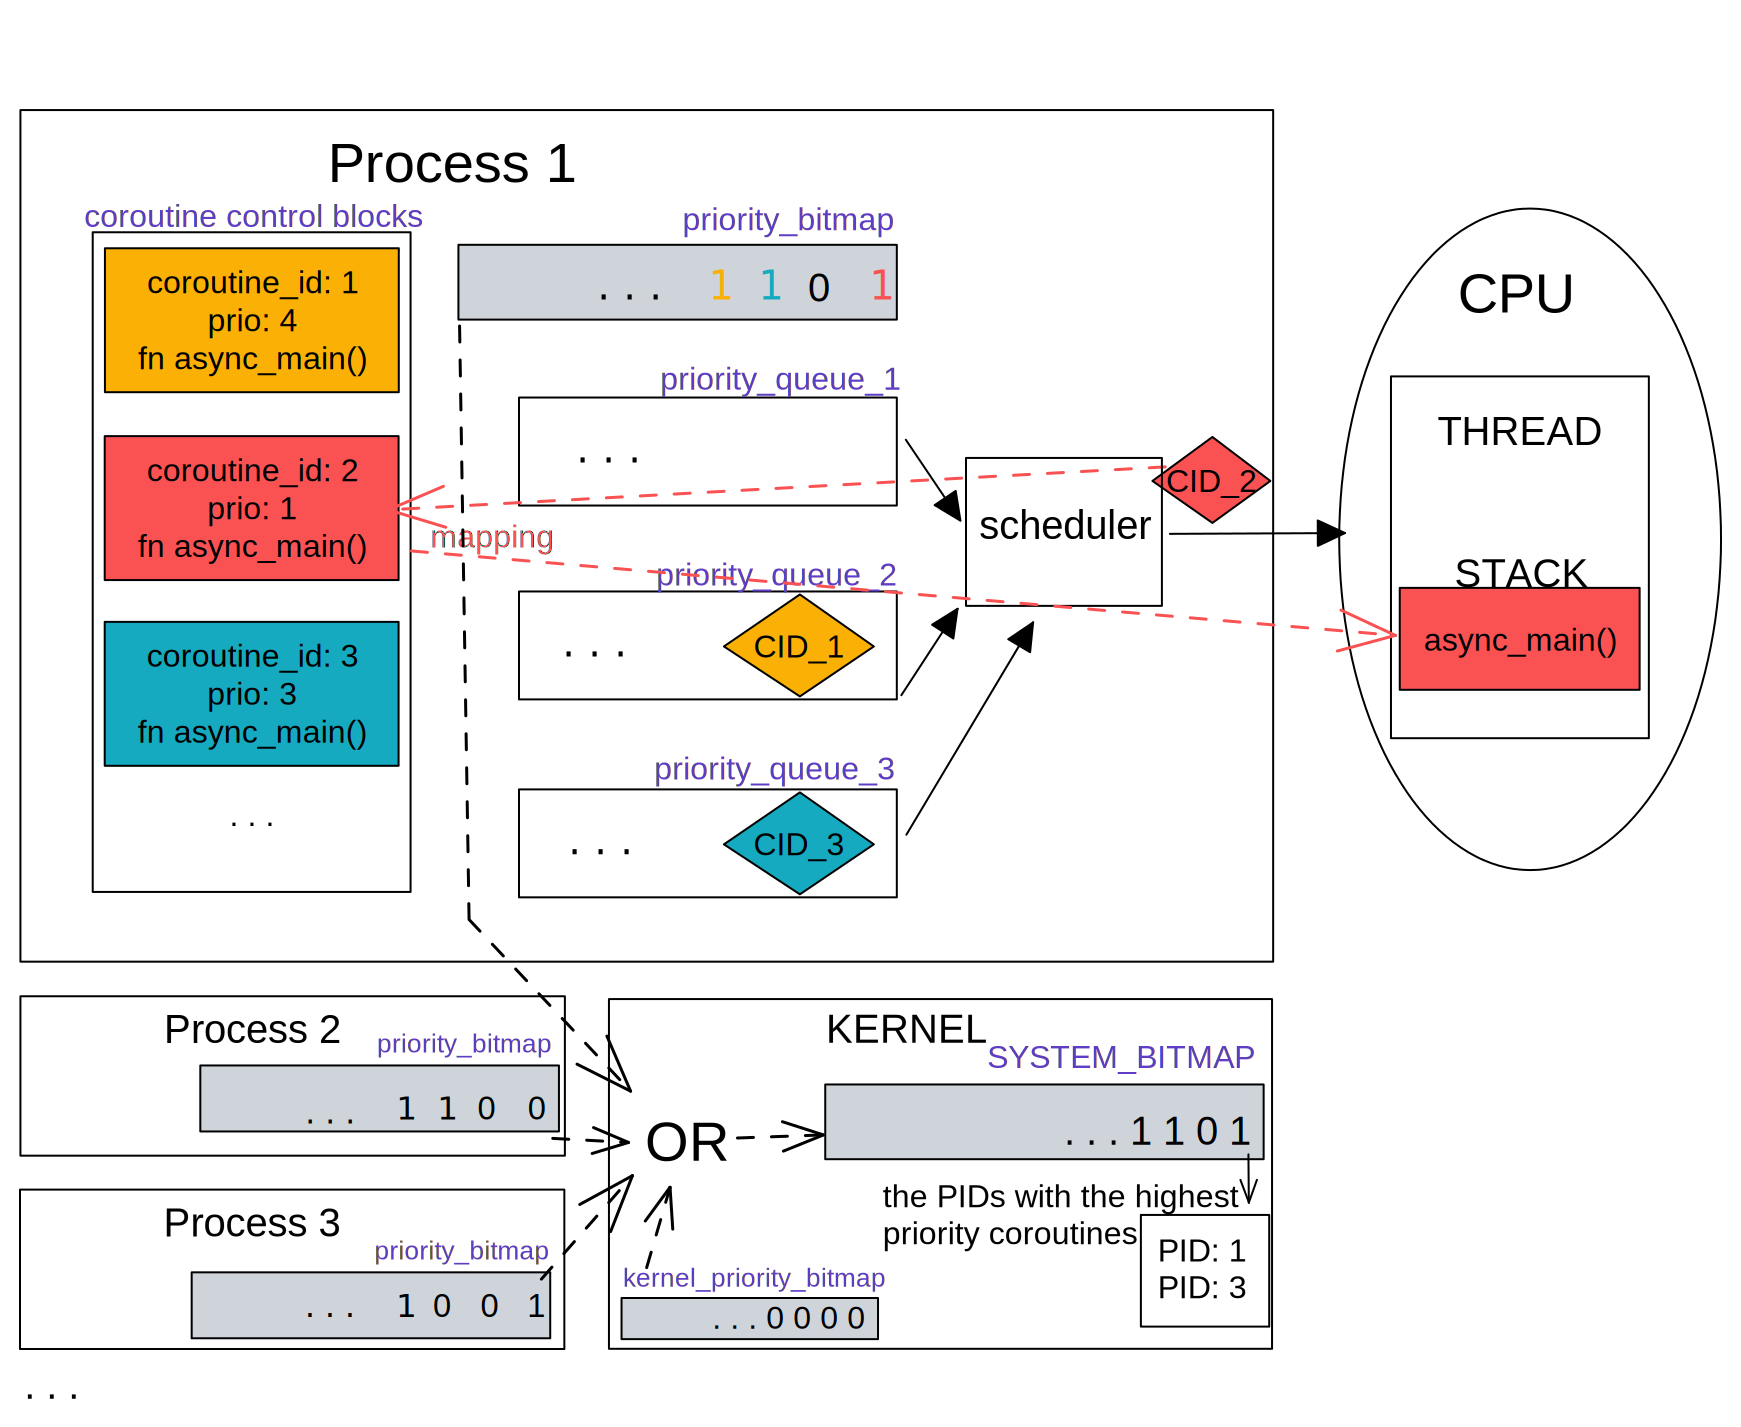
\includegraphics[width=\columnwidth]{SDSS2021-LaTEX/overview.png}
\caption{The architecture of the coroutine model in this paper}
\label{overview}
\end{center}
\end{figure}

As shown in \textit{Figure 1}, the Rust language provides asynchronous functions, and the coroutine library provides priority and coroutine ID fields and encapsulates them into a data structure called a coroutine control block. Each coroutine control block represents a coroutine. And a coroutine can be regarded as a scheduling object corresponding to a global asynchronous function one-to-one. We use the coroutine ID as an index to store all the coroutines in a hash table on the process's heap memory. By traversing this hash table, we can get all the coroutines, and we can also get or delete the specified coroutine through the coroutine ID. 

The coroutine scheduler provides two necessary interfaces: push and pop, which are used to insert and delete coroutines, and implement the coroutine scheduling algorithm. For priority scheduling, we will set up multiple queues, each with a different priority, and store the coroutine ID of the coroutine at the corresponding priority in it. Query these queues from high to low priority to complete priority scheduling. After getting a coroutine ID from the scheduler, if you need complete information of the coroutine, you can get it through the coroutine ID and the hash table. Considering that the coroutine will enter and exit the scheduler many times during its life cycle due to waiting for external events, compared to the scheduler directly managing the coroutine, this can reduce the memory overhead when the scheduler works. We use the priority bitmap to describe the priority layout of the coroutines within each process. We also use a bitmap in the kernel to describe the priority layout of the coroutines of all processes. The kernel can perceive the existence of coroutines and their priority through these bitmaps, and formulate the scheduling strategy of the process, thereby indirectly intervening in the coroutine scheduling in the user mode. This makes coroutine scheduling no longer an independent behavior within each process but allows them to be considered uniformly from a global perspective. Its design and implementation will be introduced in Section 2.3. The above is the coroutine structure within the process.

The execution of functions must depend on the stack, the same is valid for asynchronous functions. For this, we have the following design: When a coroutine needs to be executed, we start the coroutine executor, which is essentially a function. The coroutine executor will take out all the coroutines in the ready state and run them in a loop. The coroutine will use this thread's stack to execute its asynchronous function. When the coroutine is completed or suspended due to waiting for external events, it will exit the occupied thread stack by returning the function. At this time, the thread running the coroutine executor is idle. To be precise, it is not executing any coroutine, which means the next coroutine can use its stack. If there are no ready coroutines, the coroutine executor thread breaks out of the loop and ends.

The coroutine needs to be woken up after it yields because it waits for external events. Wake-up is a key mechanism of the coroutine. This part is described in detail in Section 2.4.


\subsection{Interface}
We implement this model as a function library. This library provides two interfaces, which are used to create coroutines and start coroutine executors, respectively. Since all instructions of this function library do not depend on the support of the operating system, such as system calls, both user mode and kernel mode can use these two interfaces to create and run coroutines by calling library functions.

\lstset {
    language=C++,
    frame=tb,
    tabsize=4,
    showstringspaces=false,
    numbers=left,
    %upquote=true,
    commentstyle=\color{commentgreen},
    keywordstyle=\color{eminence},
    stringstyle=\color{red},
    basicstyle=\small\ttfamily, % basic font setting
    emph={int,char,double,float,unsigned,void,bool},
    emphstyle={\color{blue}},
    escapechar=\&,
    % keyword highlighting
    classoffset=1, % starting new class
    otherkeywords={>,<,.,;,-,!,=,~},
    morekeywords={>,<,.,;,-,!,=,~},
    keywordstyle=\color{weborange},
    classoffset=0,
}

\begin{lstlisting}
// Interface1:
fn coroutine_create(async_func, priority = DEFAULT);
\end{lstlisting}

The interface \textit{coroutine\_create} for creating a coroutine requires passing in a necessary asynchronous function, which encapsulates the instructions that the coroutine needs to execute. In the Rust language, you only need to add the async keyword before the declaration of a normal function to declare it as an asynchronous function. In addition, you can specify the priority of the coroutine in the parameter. If not specified, the priority of the coroutine will be set to the default value. The interface will encapsulate the incoming asynchronous function as a coroutine, and insert it into the coroutine queue of the corresponding priority, waiting to be scheduled for execution.

\begin{lstlisting}
// Interface2:
fn coroutine_run(wait);
\end{lstlisting}

Start the coroutine executor interface \textit{coroutine\_run} to jump to the function responsible for scheduling and executing the coroutine. When there is no coroutine in the process (no coroutine has been created or all coroutines have been executed), this interface will exit immediately. And when there is no coroutine in the ready state in the process, but there is at least one coroutine in the waiting state, you can choose to exit the interface through the passed in parameters, or wait for the appearance of the coroutine in the ready state.


\subsection{Priority and Schedule}

We handle the scheduling order of coroutines based on priority. Within a process, coroutines are executed from high to low priority; between processes, the process with the highest priority coroutine will be scheduled first. The scheduler only operates on the coroutine ID to simplify memory operations. When the complete information of the coroutine is required, it can be obtained by mapping the coroutine ID.


\subsubsection{Coroutine scheduling within a process}

Each coroutine has a priority. The IDs of coroutines at the same priority are managed by the same queue. Multiple different priorities will correspond to multiple different queues, they form a queues group. Each process has only such a group, which is stored in the process's heap memory. The coroutines in the priority queues are all in a ready state, that is, they can be scheduled for execution immediately, but the order of execution is distinguished by priority. Obviously, the newly created coroutine will be inserted directly into the queue. For non-ready coroutines, they will be re-inserted into the priority queue after being woken up. The specific process will be introduced in Section 2.4.

At any position in any thread, we can call the \textit{coroutine\_run} interface mentioned in Section 2.2 to execute the coroutine. It will continuously access the scheduler in a loop to get the coroutines and execute them. At this time, the scheduler will access the queues from high to low according to priority. , when the first non-empty queue appears, a coroutine ID is popped from the queue, and this coroutine is one of the highest priority coroutines that can be executed immediately in the process.

If all queues are empty, no coroutines can be executed in the process, and the scheduler will return an empty value. At this time, it will be further judged whether the number of coroutines is 0, that is, whether there are coroutines in the waiting state. If there is no coroutine, it means that all the coroutines are executed, and the coroutine executor can be exited. If there is, choose to exit the \textit{coroutine\_run} function according to the parameters passed in, or call the system call to make the current thread yield until it is rescheduled and at least one ready coroutine exists to continue the execution of coroutines



\subsubsection{Coroutine Scheduling of the Whole System}

Based on the previous design, the priority scheduling of coroutines can be implemented within the process. Now, we extend it to the entire system to perform priority scheduling on the coroutines of all processes. This requires obtaining the priority information of the coroutines of all processes in the kernel and recording the process of the coroutine with the highest priority. Then when switching from the kernel to the user mode, the process is scheduled, and the highest priority coroutine can be scheduled to run in the process.


\paragraph{Priority Bitmap}~{}

We use bitmaps to describe the priority layout of coroutines.

Each process will maintain a bitmap whose length is the number of priorities of the coroutines, and the value of each bit is 0 or 1, indicating whether there is a coroutine of that priority. When accessing the scheduler to insert or require a coroutine, the queue corresponding to the priority will push or pop a coroutine ID. If it changes from empty to non-empty or non-empty to empty, the corresponding bit in the process bitmap is written as 1 or 0.

Since the kernel also has its own address space, it can create and run coroutines. Therefore, the kernel also has a priority bitmap to represent the priority information of the coroutines it manages, called the kernel bitmap.

In addition, we set an extra bitmap in the kernel to represent the priority information of the coroutines of the whole system, which is called the system bitmap. The length of this bitmap is also the number of priorities of the coroutines. Still, the 0 or 1 of each bit represents whether there are coroutines of this priority in all processes of the entire system. To calculate the value of this bitmap, it is necessary to enable the kernel to access the bitmaps of all processes. Our approach is to specify a virtual address as the address of the process accessing the bitmap in user mode. Then, when the process is initialized, apply to the kernel for a free physical page, map the specified virtual address to the starting address of the physical page, and grant the process permission to read and write this address. In this way, the process can read and write the bitmap in user mode, and the kernel can also directly access the bitmap of the process.

We map each process ID with the physical address of its process bitmap, and we can get all process bitmaps in the kernel by enumerating the IDs of the processes.

\begin{figure}[ht]
\begin{center}
\centerline{\includegraphics[width=\columnwidth]{bitmap.png}}
\caption{The structure of priority bitmaps in the kernel}
\label{bitmap}
\end{center}
\end{figure}

The value of the system bitmap is based on all process bitmaps. When the clock interrupt arrives, the kernel is responsible for traversing the bitmaps of all processes and updating the system bitmap. However, it is evident that this calculation process is a relatively simple procedure, that is, it only needs to perform OR operations on all process bitmaps-as long as at least one coroutine of at least one process belongs to this priority, the corresponding bit in the system bitmap is 1, and only when all processes do not have coroutines of this priority, the corresponding bit in the system bitmap will be 0. The update is completed by assigning the results of the OR operations of all process bitmaps to the system bitmap.

\paragraph{Global Scheduling Based on Priority Bitmap}~{}

The current system has process bitmaps and the system bitmap, which can schedule the process with the highest priority coroutine after each clock interrupt. Within a clock interrupt, the bitmap of the process will change as the coroutines are created and exited. Still, the bitmap changes of each process will not be synchronized to the system bitmap before the next clock interrupt. That is to say when all the highest priority coroutines return (exit or yield) and before the next clock interrupt arrives, the priority scheduling of coroutines is not yet satisfied for the entire system. If we want all coroutines of the whole system to abide by priority scheduling during operation strictly, we further provide the following design.

As we know, the coroutine will yield the thread stack by exiting or yielding via function return. In either case, it will enter the next loop after that and access the scheduler again to obtain a coroutine and execute it. Before entering the next loop, we can read the process bitmap and the system bitmap and compare the highest priority recorded by the two, which is equivalent to querying whether there are unexecuted highest priority coroutines in this process. If the highest priority of the coroutine in the process is lower than the highest priority of the coroutine in all processes recorded in the system bitmap, It means that the highest priority coroutines in this process have all been executed. At this time, the system call \textit{sys\_yield} should be called to yield the current processor, enter the kernel to update the system bitmap, and schedule according to the result; otherwise, continue to execute.

Obviously, if strict priority scheduling is pursued, a large amount of switching overhead between user mode and kernel will be introduced due to updating the system bitmap multiple times during a clock interrupt. So this way should be offered as an option. Since this is the behavior of the coroutine executor (it decides whether to check the system bitmap), we can control whether it is turned on or not through a parameter. By default, relaxed priority scheduling is performed, that is, schedule the process with the highest priority coroutine only after each clock interrupts, and the system bitmap is not updated within a clock interruption.


\subsection{Excutor and Asynchronization }

The executor is the coroutine management organization in this model, responsible for managing the coroutine data structures, priority queues, and the coroutine wake-up mechanism described in this section.

\begin{figure}[ht]
\begin{center}
\centerline{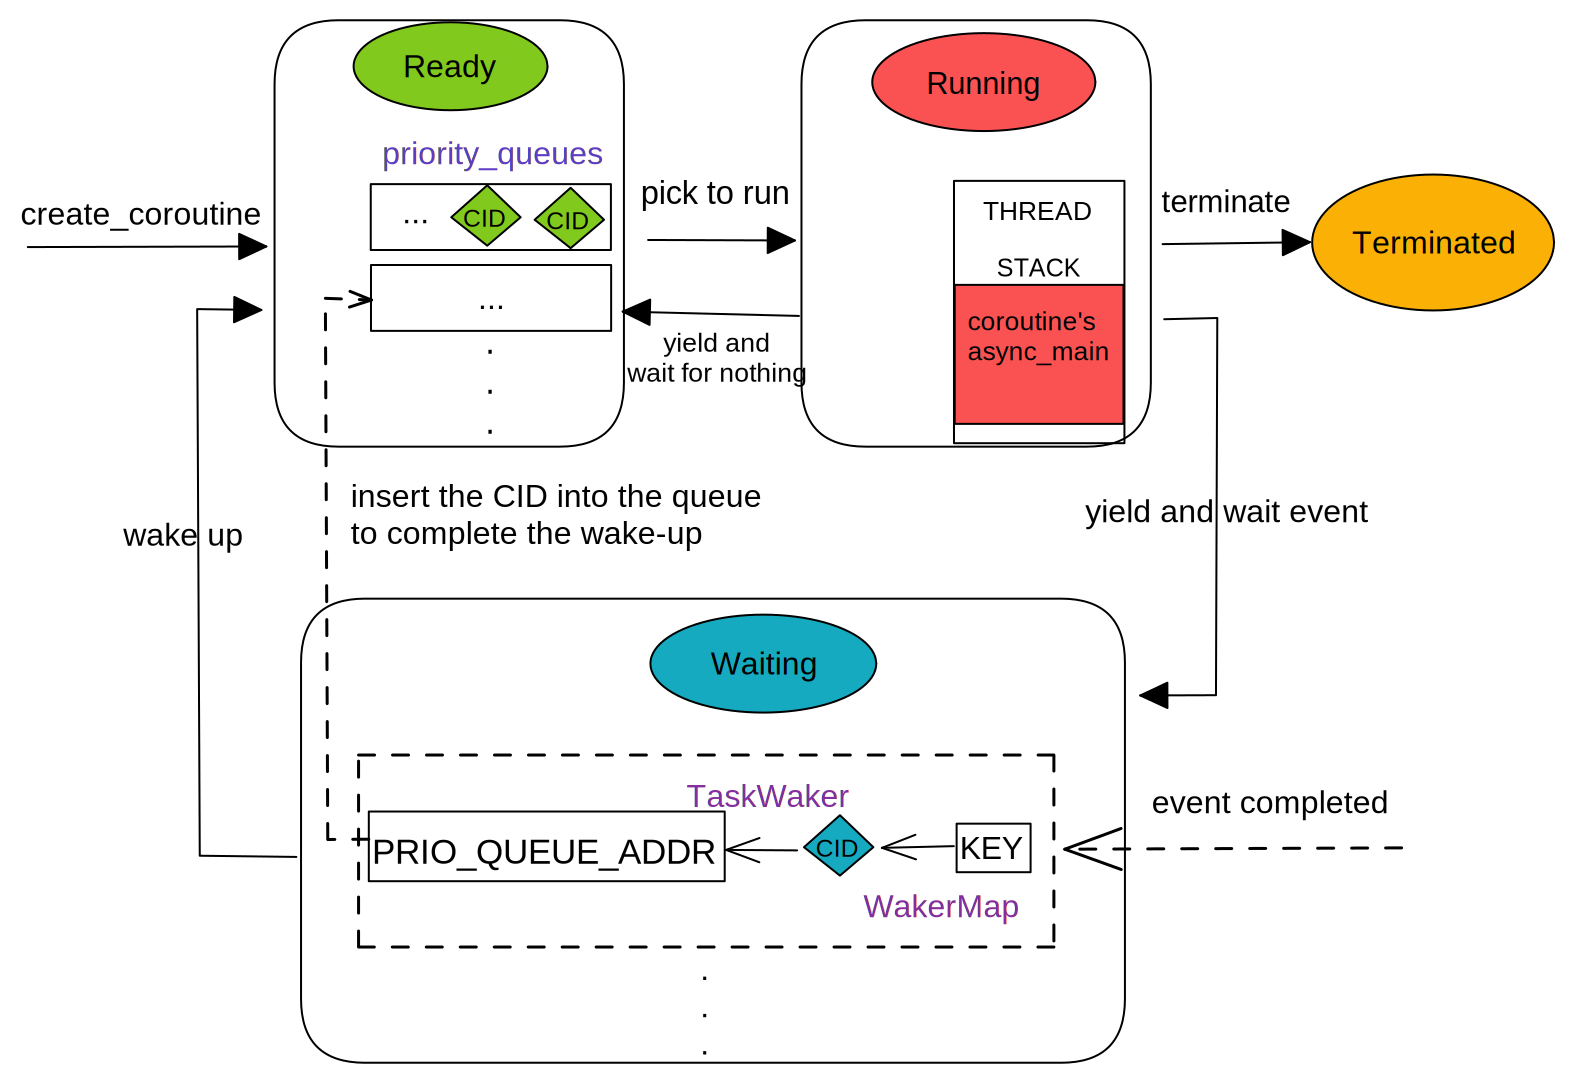
\includegraphics[width=\columnwidth]{states.png}}
\caption{The state transitions of a coroutine during its lifetime}
\label{states}
\end{center}
\end{figure}

Let's take a closer look at the two situations in which coroutines give up the thread stack:

1. After the coroutine is executed, the main function of the coroutine is executed and returned. At this time, the data structure of the coroutine will be found according to the coroutine ID and the heap memory occupied by it will be released;

2. The coroutine has not been executed and cannot continue to execute because it is waiting for an external event, so it chooses to give up by returning the function. At this time, we advocate not inserting the coroutine ID back into the priority queue but directly entering the next round of loops and accessing the scheduler to take out the next coroutine and execute it. When the waiting event of the suspended coroutine arrives, the wake-up operation is performed, that is, the wake-up coroutine ID is inserted back into the priority queue. This is the asynchronous mechanism of the coroutine in this model. It can complete the wake-up operation of the coroutine conveniently and ensure the work efficiency of the scheduler. This means that each coroutine in the priority queues is in a ready state that can be executed immediately. When accessing the priority queues, there is no need to check the coroutine's state nor to access the coroutine in the waiting state.

Now we know that the operation of waking up a coroutine is to insert the ID of the coroutine into the corresponding priority queue, which requires the ID of the coroutine, the priority of the coroutine, and the address of the priority queue. We can encapsulate these three variables into a data structure called \textit{TaskWaker}, and establish a mapping between the coroutine ID and the corresponding \textit{TaskWaker}. When a coroutine needs to be woken up, only its coroutine ID is needed. For the creation timing of TaskWaker, we can check whether the TaskWaker is created before the coroutine is selected to execute and has not yet started to execute. If not, create it and hand it over to the Executor for management. Obviously, when a coroutine exits, its corresponding taskwaker is deleted immediately.

So the key question now is how to get the coroutine ID waiting to be woken up for the coroutine that executes the waiting event and the wake-up operation. We introduce a data structure called \textit{WakerMap} here, which maintains the mapping of integer key values to coroutine IDs. For the waiting coroutine and the coroutine that performs the wake-up operation, they need to pass in the same key value when they are created (this requires the use of a global counter with mutually exclusive access within the process) to establish a connection. When the coroutine waits for an external event, the key-value pair consisting of the integer passed in the parameter and the coroutine ID is inserted into the WakerMap, and then when another coroutine completes the external event, it can directly find the one that needs to be awakened according to the key value; If the coroutine that performs external events and wake-up operations is scheduled to execute first, it will find empty items and do nothing when it queries WakerMap to wake up another coroutine, but this does not affect the execution of the program. Later, when the coroutine waiting for the external event is executing, it will find that the waiting event has already arrived (for example, the buffer has written enough data), and will not return and yield the thread stack

Based on the above design and implementation, we can summarize the coroutine scheduling of this model as considering the coroutines in the ready state in the entire system (including user mode and kernel), the process with the highest priority coroutine will be entered from the kernel after each clock interrupt. The priority scheduling of coroutines is then performed within that process. If there is a coroutine with a higher priority in user mode than in kernel, the user mode program will be scheduled for execution first.


\section{PERFORMANCE COMPARISON}

We introduced this coroutine library on rCore OS, which enables rCore to create and execute coroutines. On this basis, experiments are designed to compare the performance difference between the rCore that uses coroutines and the unmodified rCore that uses threads.

\subsection{Experiment A: Test in User Mode without the Syscall}

This experiment uses coroutines or threads to make ordinary function calls in user mode, and does not use system calls and does not involve the kernel.

The experimental steps are as follows:

1. This experiment is created as processes, and each process creates N coroutines or threads to do the same work. These N coroutines or threads are numbered from 1 to N, and the value of the number is passed in as a parameter. Get a start time when the process starts, get an end time before the process exits, and use the time difference between the two as their total execution time;

2. Each coroutine or thread will mutually exclusive read and write a global variable, execute the read first, and execute the write after the read is successful. The initial value of the global variable is set to 0. When the value of the global variable read by the coroutine or thread is equal to its own number, it is considered that the reading is successful, and then the write operation is performed, that is, the value of the global variable is incremented by 1. When all coroutines or threads are created, the main thread adds 1 to the global variable so that the coroutine or thread numbered 1 can start reading and writing. It also enables subsequent coroutines or threads to be started.

3. When the reading is unsuccessful, the coroutines yield the thread stack according to the asynchronous mechanism and wait to be woken up; the thread calls the system call to perform thread switching.

4. In this experiment, the concurrency of coroutines or threads is increased from 200 to 4000, and the step size is 200;

\begin{figure}[ht]
\begin{center}
\centerline{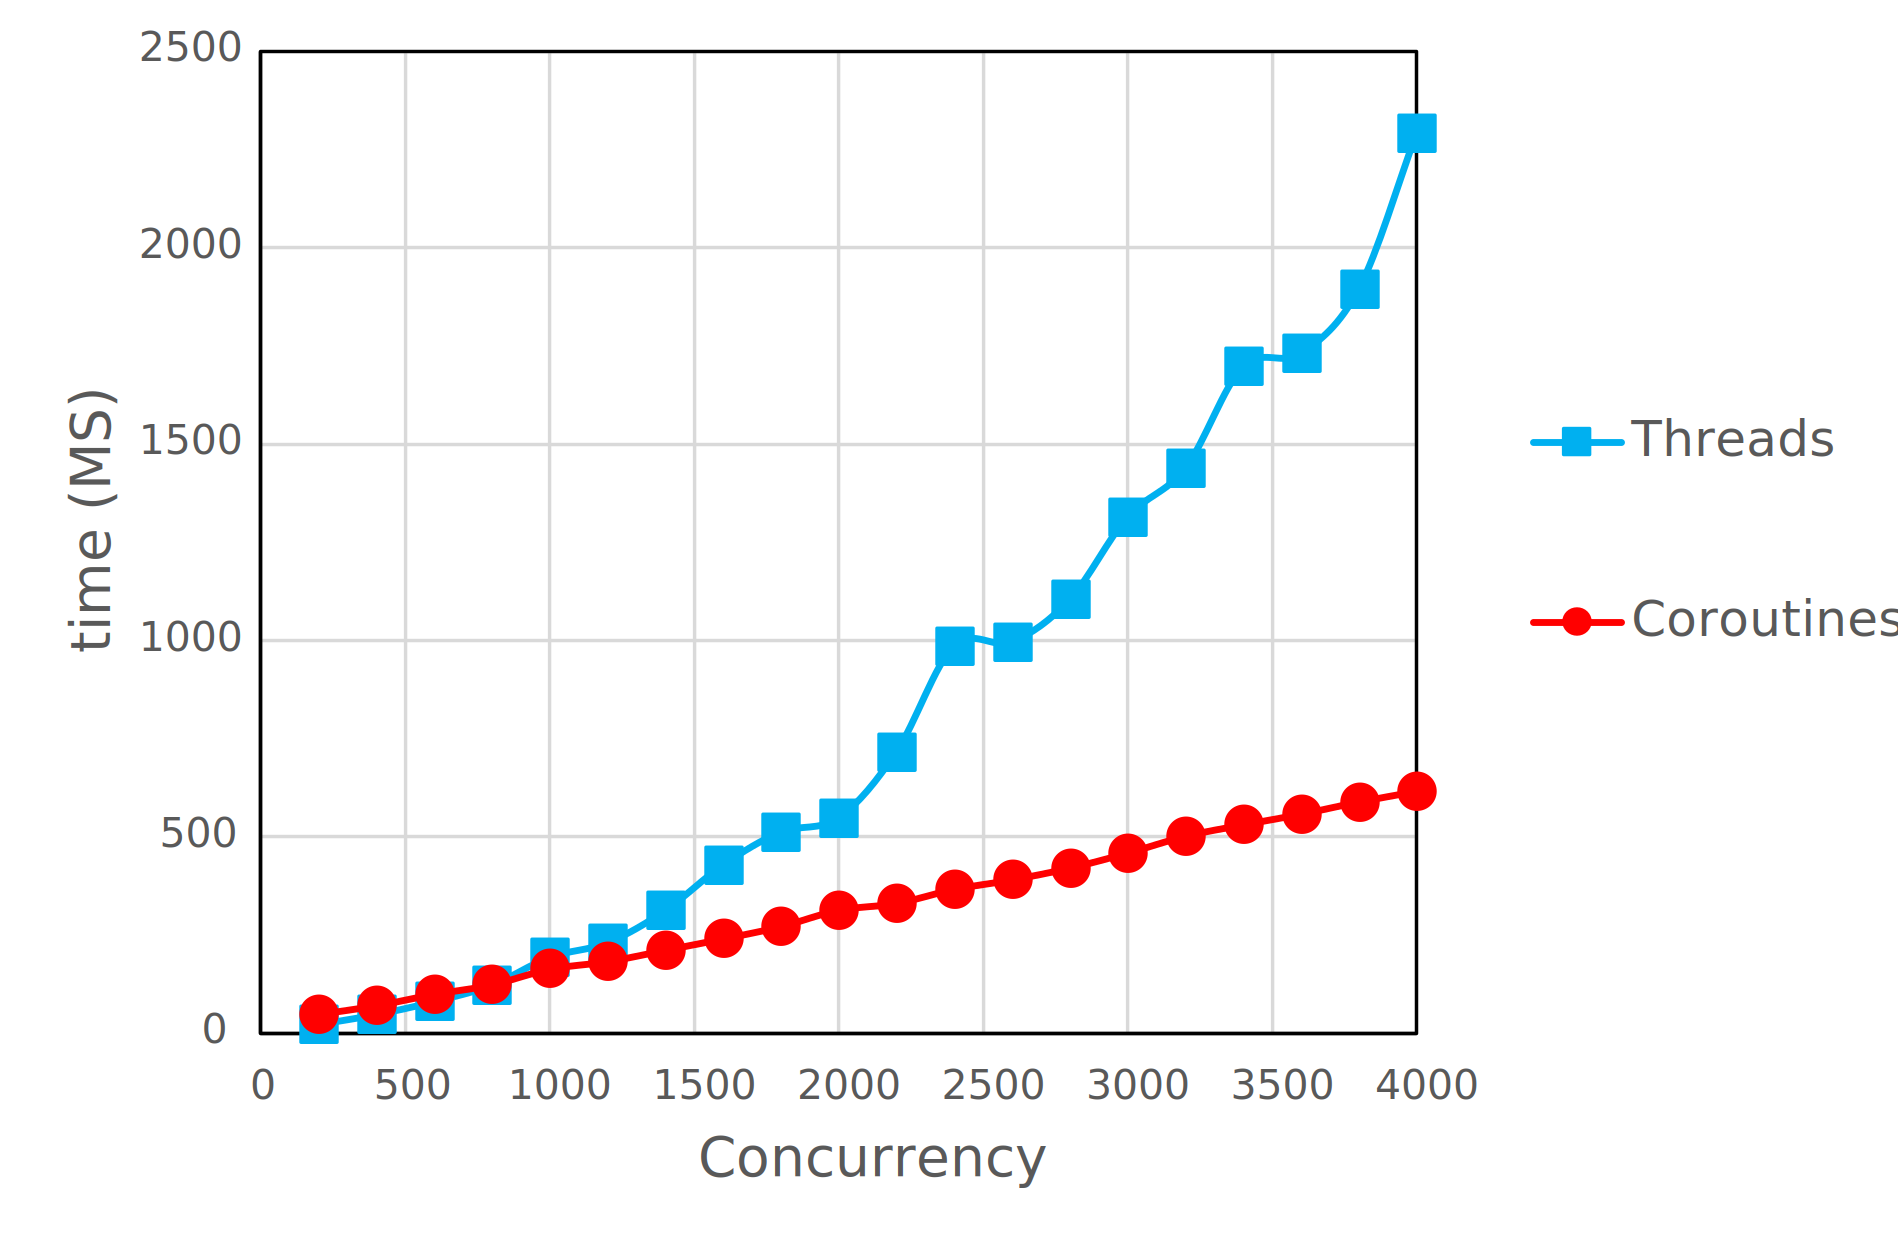
\includegraphics[width=\columnwidth]{user.png}}
\caption{Performance comparison of coroutines and threads in user mode}
\label{user}
\end{center}
\end{figure}

\begin{figure}[ht]
\begin{center}
\centerline{\includegraphics[width=\columnwidth]{user_table.png}}
\caption{Test data of key nodes, including starting point, ending point, and the turning point where the coroutine performance exceeds the thread}
\label{user_table}
\end{center}
\end{figure}

As can be seen from [Figure 5], when the concurrency is small, the total execution time of coroutines is greater than that of threads. The total execution time of coroutines increases steadily as the number of concurrency increases, while the total execution time of threads increases rapidly and exceeds that of coroutines. It can be seen from [Table 1] that at the beginning of this experiment, that is, when the concurrency is 200, the performance of coroutines is weaker than that of threads; When the concurrency is greater than or equal to 800, the performance of the coroutines begins to exceed that of the threads; when the maximum concurrency of the test is 4000, the total execution time of the coroutine is about 26\% of the thread.

\subsection{Experiment B: Test in user mode with syscall}

This experiment is carried out in user mode, and each coroutine or thread will use read and write system calls, so this experiment involves the kernel. This experiment is carried out in user mode, and each coroutine or thread will use read and write system calls to enter the kernel. 

\begin{figure}[ht]
\begin{center}
\centerline{\includegraphics[width=\columnwidth]{test2.png}}
\caption{experiment B, the read and write ends of the pipe are located in two coroutines or threads, respectively.}
\label{test2}
\end{center}
\end{figure}

The experiments we designed are shown in \textit{Figure 6}. The experimental steps are as follows:

1. This experiment is created as processes, and each process creates N coroutines or threads to do the same work. These N coroutines or threads are numbered from 1 to N, and the value of the number is passed in as a parameter. Get a start time when the process starts, get an end time before the process exits, and use the time difference between the two as their total execution time;

2. We create N+1 pipes, numbered from 1 to N+1, pipes can be read and written by different coroutines or threads. The working method of the used pipe is: only when the write end is closed, the read operation of this pipe can read the data and then complete the read operation; when the write end is not closed, the read operation will cause thread switching in the kernel;

3. Each coroutine or thread reads and writes to the pipes. Specifically, the coroutine or thread numbered i (1<= i <= N) will read data from the pipe numbered i. After its write end is closed, the coroutine or thread can successfully read the data, then write data to the pipe numbered i + 1 and close the write end of the pipe numbered i + 1. Then the work of this coroutine or thread is completed, and the coroutine or thread numbered i + 1 can start the read operation. It is equivalent to using pipes to connect all coroutines or threads in series, and the read and write operations to the same pipe are located in two adjacent coroutines or threads.

4. After all coroutines or threads are created, the main thread of the test program will directly write data to pipe 1 and then close its write end. After that, with the scheduling and execution of coroutines or threads, the data will be read from the pipe numbered 1 by the coroutine or thread numbered 1, and then written to pipe 2, and the coroutine or thread numbered 2 will read the data from pipe 2, and then write to pipe 3, and so on;

5. Pipes read and write the same amount of data per test. We tested coroutines and threads on three data sizes of 1B, 256B, and 4096B, respectively.

6. In the experiment, the concurrency of coroutines and threads is increased from 200 to 4000, and the step size is 200;

\begin{figure}[ht]
\begin{center}
\centerline{\includegraphics[width=\columnwidth]{1B.png}}
\caption{The amount of data read and written by the pipe is 1B}
\label{1B}
\end{center}
\end{figure}

\begin{figure}[ht]
\begin{center}
\centerline{\includegraphics[width=\columnwidth]{256B.png}}
\caption{The amount of data read and written by the pipe is 256B}
\label{256B}
\end{center}
\end{figure}

\begin{figure}[ht]
\begin{center}
\centerline{\includegraphics[width=\columnwidth]{4096B.png}}
\caption{The amount of data read and written by the pipe is 4096B}
\label{4096B}
\end{center}
\end{figure}

\begin{figure}[ht]
\begin{center}
\centerline{\includegraphics[width=\columnwidth]{1B_table.png}}
\caption{Test data of key nodes with 1B data volume}
\label{bayespic}
\end{center}
\end{figure}

\begin{figure}[ht]
\begin{center}
\centerline{\includegraphics[width=\columnwidth]{256B_table.png}}
\caption{Test data of key nodes with 256B data volume}
\label{256B_table}
\end{center}
\end{figure}

\begin{figure}[ht]
\begin{center}
\centerline{\includegraphics[width=\columnwidth]{4096B_table.png}}
\caption{Test data of key nodes with 4096B data volume}
\label{4096B_table}
\end{center}
\end{figure}

It can be seen from \textit{Figure 7, 8, 9} that when the concurrency is small, the total execution time of coroutines and threads is very close. As the amount of concurrency increases, the total execution time of threads increases rapidly and exceeds that of coroutines. It can be seen from \textit{Figure 10, 11, 12} that in this experiment when the concurrency is 200, the performance of the coroutine is weaker than that of the thread; when the concurrency is greater than or equal to 400, the performance of the coroutine begins to exceed that of the thread; When the tested maximum concurrency of 4000 is reached, the total execution time of the coroutines is about \textit{32\% - 44\%} of the threads.

Through experiments we can see that the performance of coroutines is not necessarily better than threads in all cases. When the amount of concurrency is small, the basic overhead of supporting the coroutine running, including the coroutine scheduler and the wake-up mechanism, has a significant impact, resulting in the performance of the coroutine at this time being close to that of the thread. However, as shown in the experimental data, the usage overhead of coroutines increases linearly with the increase of concurrency, which means that the increase of concurrency does not significantly impact the average execution time and average switching time of coroutines. This is a distinguishing feature of coroutines from threads and also the significance of coroutines for concurrent programming. In contrast, the context switching cost of threads increases with the increase of concurrency, which causes the performance of coroutines to gradually exceed threads when the amount of concurrency increases, and the gap between the two becomes larger and larger.

\section{Conclusions}

This paper proposes and implements a coroutine model based on Rust language features. A Rust operating system can use this coroutine library to create and run coroutines that support priority scheduling in user mode and the kernel.  Based on the O(1) scheduling algorithm of Linux, we designed the coroutine priority bitmap of the process and the coroutine priority bitmap of the kernel, so that the scheduling of coroutines is no longer an independent behavior within each process, but can be controlled by the kernel. This allows some time-sensitive coroutines to be scheduled preferentially in the entire system, while some time-insensitive coroutines can be set to a lower priority, reducing competition with high-priority coroutines, so that the processor can be assigned more flexibly and scientifically.

We have introduced this coroutine library on rCore OS and conducted performance comparison experiments. Experimental results show that the performance of coroutines is not necessarily better than threads in all cases. When the amount of concurrency is small, the execution time of coroutines will be longer than that of threads. This is because the basic overhead required to run coroutines, such as scheduling, switching, and wake-up, significantly impacts the coroutines when the number of concurrency is small. However, as the amount of concurrency increases, the overhead required for coroutines to run grows slowly while threads grow rapidly, so the gap between the two continues to grow. When the concurrency is greater than 200 - 800, the execution time of the threads gradually exceeds that of the coroutines. When the concurrency reaches 4000, the total execution time of the coroutines is about \textit{26\% - 44\%} of the threads.

\bibliographystyle{plain}
%% Define a new 'leo' style for the package that will use a smaller font.
\makeatletter
\def\url@leostyle{%
  \@ifundefined{selectfont}{\def\UrlFont{\sf}}{\def\UrlFont{\small\ttfamily}}}
\makeatother
%% Now actually use the newly defined style.
\urlstyle{leo}


\bibliography{ref}

\end{document}
